In the last years the interest among data-intensive technologies and applications in order to extract useful information from data has increased in our day to day. These data-intensive applications and their execution environments allow users not only to handle Big Data but also to do it efficiently. This is why Big Data has become in a common technology in our lives.

Furthermore, the appearance of Big Data has generated some needs in our society. One of these needs is privacy policies. DIAs require some tools which are able to preserve the privacy of users which are generating such data. These tools can vary from international laws that legislate in this regard to technical approaches that allow to encrypt the flowing data.

Due to the development of dataflow applications and the wide range of fields where Big Data is still getting involved, writing DIA codes from scratch became in an inefficient task. At this point was where modeling techniques for software development became important for DIA development. StreamGen is an example of a platform used to develop DIAs from UML class diagrams by means of Papyrus. However, StreamGen does not allow to specify privacy policies.

Some approaches can be found in the literature about privacy policies applied to dataflow applications as it is the case of \cite{privacypoliciesarticle}. This approach allows to specify two different types of privacy policies: View Creation Policies and Data Subject Eviction Policies. Each of these privacy policies are determined by means of a transformation in charge of each of the policies. Moreover, a past condition checker operator is considered in order to check not only the static context variables conditions specified by the user but also some conditions about the variables flowing through the streams of the DIA which could be given in the past. Moreover, this article introduces a source generating the viewer tuple (SCV tuples) to feed the privacy operators.

In \cite{privacypoliciesarticle} a dataflow application based on an e-commerce example is presented to explain how privacy policies could be applied to StreamGen. Such application consists of three operators to compute some real time statistics about the transactions generated by the consumers of the e-commerce company. The statistics are sent to external companies in order to provide useful information to both parts, the clients and the external company that buys the statistics.

In order to develop this, a source, three transformations and three sinks are connected by means of streams as can be seen in the figure \ref{fig:Great Seller Dataflow Model}. This figure represents the dataflow model of the application without any privacy policy.

\begin{figure}
\centering
{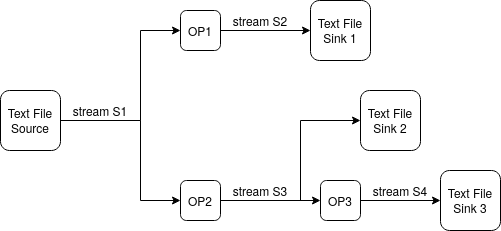
\includegraphics[scale=0.3]{./chapter3/greatSellerApp.png}}
\caption{Great Seller Dataflow Model}
\label{fig:Great Seller Dataflow Model}
\end{figure}

Once the application is developed, in \cite{privacypoliciesarticle}, an algorithm is presented in order to generate the privacy-aware dataflow application. Such algorithm is able to generate two privacy policies, a VCP and a DSEP:

\begin{itemize}
\item VCP: the client avoids that the employees of a market consultancy (MarketConsult employees) know if the client spent amount in the last 30 minutes is bigger than \euro{100} and if the number of issued transactions by the client is bigger than 3, in such case, the spent amount should be modified to the biggest allowed (\euro{100}).
\item DSEP: the client does not allow that data goes to one of the operators (to operator 3) when MarketConsult observes the application.
\end{itemize}

In order to do this, some specific privacy policy operators are introduced. Such privacy policy operators are:

\begin{itemize}
\item StaticContextSource.
\item PastConditionChecker.
\item ViewBuilder.
\item DataSubjectEvictor.
\end{itemize}

The proposed algorith in \cite{privacypoliciesarticle} works with these operators as follows. First of all, the algorithm takes as input the application which is not privacy-aware. Moreover, when the algorithm is called, a StaticContextSource is directly added to the input application. Such source introduces the external companies which apply for the statistical information. After that, depending on the stream, if it is VCP-aware or DSEP-aware, a ViewBuilder operator (VCP-aware stream) or a DataSubjectEvictor operator (DSEP-aware) are added to the input application. Finally, if any past condition must be taken, a PastConditionChecker operator is applied over the corresponding stream. In the e-commerce example that is specified above, the stream S2 is VCP-aware and DSEP-aware then a ViewBuilder operator and a DataSubjectEvictor operator are applied on such streams and added to the non-privacy-aware- application. Moreover, a past condition is applied for the stream S2 then a PastConditionChecker is applied on the stream S2 and added to the input application. In the figure \ref{fig:Great Seller Privacy Dataflow Model} can be the seen the privacy-aware dataflow model of the e-commerce application after applying the algorithm presented in \cite{privacypoliciesarticle}.

\begin{figure}
\centering
{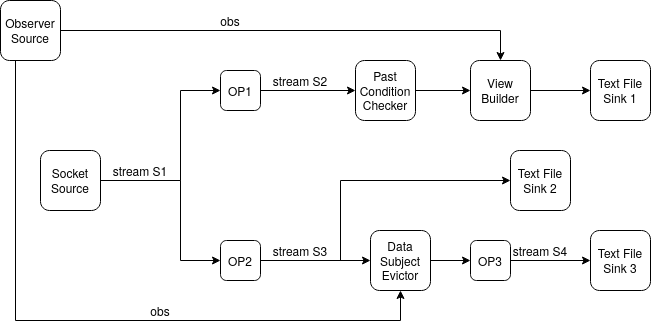
\includegraphics[scale=0.3]{./chapter3/greatSellerPriv.png}}
\caption{Great Seller Privacy Dataflow Model}
\label{fig:Great Seller Privacy Dataflow Model}
\end{figure}

All the Java files developed to implement the privacy-aware e-commerce application are uploaded in two GitHub repositories (\url{https://github.com/MicheleGuerriero/dataflow-privacy-library/tree/master/src/main/java/it/deib/polimi/diaprivacy/library} and \url{https://github.com/MicheleGuerriero/common/tree/master/src/main/java/it/deib/polimi/diaprivacy/model}). Such files are stored there with the goal to provide a library to future developers to apply VCP and DSEP privacy policies in dataflow applications.

As it can be seen, this approach requires that dataflow application developers have some knowledge about the privacy policy language but also about the targeted platform language (Hadoop, Spark, Flink...) which supposes a loss of speed to design DIAs. These inefficiencies are given due to the fact that, after implementing the application without privacy policies, the privacy policy operators are not developed among the StreamGen language and neither the translation from the UML language to the target language. Then, there is no possibility to apply the presented algorithm in an easy way. Because of this, the current document faces the following objectives:

\begin{itemize}
\item To extend the StreamGen high level modeling approach to enable the modeling of privacy-aware streaming applications.
\item To allow software developers with few knowledge about privacy policies to handle the design of privacy-aware streaming applications.
\item From a non-privacy-aware application reach a privacy-aware application easily.
\end{itemize}

Thus, first of all, the StreamGen high level modeling approach, which is defined by means of a UML profile diagram, must be modified in order to add all the elements which are necessary to design privacy-aware streaming applications. Moreover, the reached profile must be elegantly integrated with the current profile. In order to achieve this goal, a new language that slightly differs from the language of the four operators presented in \cite{privacypoliciesarticle} is defined. The new language identifies which are the streams that must be protected by means of a stereotype that also has two properties to identify if the stream is VCP-protected or DSEP-protected. The extension of the language is made by means of the Eclipse plugin Papyrus. Further information about the versions used for Eclipse or Papyrus can be found in the table \ref{Program Versions Used}.

Secondly, the designer of the data-intensive application must be able to generate automatically all the Flink codes that are necessary taking into account that such designer could have few knowledge about privacy policies. In order to reach this goal, all the Acceleo codes to compile the previously defined language are written calling to the already developed library in \cite{privacypoliciesarticle}. This allows to have the same target Flink codes independently of the DIA and, then, the Flink privacy code modification by the developer is not required. For further information about the Acceleo version see the table \ref{Program Versions Used}

Finally, the new language must be easily applicable over non-privacy-aware applications in order to reach Flink codes without errors. This goal is achieved by means of an intuitive language based on the datatype package already implemented in StreamGen.

\begin{table}[h!]
\centering
	\begin{tabular}{||c|c||} 
	\hline\hline
	Program & Version \\ [1ex] 
	\hline\hline
	Eclipse & 2019-03 (4.11.0)  \\
	\hline
	Papyrus & SysML 1.4 Feature 1.3.0  \\
	\hline
	Acceleo & 3.7.8.201902261618  \\
	\hline
	m2e-Maven Integration for Eclipse & 1.11.0.20190220-2119  \\
	\hline
	Apache Flink & 1.4.0  \\
	\hline\hline
	\end{tabular}
\caption{Program Versions Used}
\label{Program Versions Used}
\end{table}

